
The results are presented in figure \ref{fig:alignment}-\ref{fig:improved_assk} and tables \ref{tab:appendix_skk_ngk}-\ref{tab:appendix_ssk_n}

Due to very high computational costs for some of the algorithms, both in time and memory, we were  not able to average over ten iterations as \cite{lodhi} did for every entry in the tables. We have clearly stated in the tables how many iterations were performed for that data. 



%2 big tables
\begin{table}
	\small
	\centering
	\subfloat[n=5]{\raisebox{0 cm}%
		{\begin{tabular}{| c | c | c | c | c | }
			\hline SSK &$ \lambda  $& Precision & Recall & $ F_1 $   \\ \hline	
			
			& 0.01 & 0.96 & 0.92 & 0.94  (0.873)   \\ 
			& 0.05 & 1 & 0.92 & 0.96 (0.882)   \\ 
			acq & 0.1 & 1& 1 &  1 (0.871)  \\
			& 0.5 & 0.89 & 1 & 0.94 (0.867)   \\ 
			& 0.7 & 0.93 & 0.96 & 0.94 (0.805)    \\ 
			& 0.9 & 0.64 & 0.96 & 0.77   (0.735)  \\ \hline
			
			
			& 0.01 & 0.95 & 0.95 &  0.95  (0.946)  \\	
			& 0.05 & 1 & 0.98 &  0.99  (0.946)  \\ 
			earn & 0.1 & 0.98 & 1 &  0.99  (0.944)  \\ 
			& 0.5 & 1 & 0.90 &  0.95  (0.936)  \\ 
			& 0.7 & 1 & 0.90 &  0.95  (0.928)  \\
			& 0.9 & 0.95 & 0.88 &  0.91  (0.914)  \\\hline
			
			
			
			& 0.01 & 1 & 0.80 & 0.89  (0.845)   \\ 
			& 0.05 & 1 & 0.87 & 0.93  (0.834)   \\ 
			corn & 0.1 & 1 & 0.87 & 0.93  (0.827)   \\ 
			& 0.5 & 0.94 & 1 &  0.97 (0.779)  \\ 
			& 0.7 & 1 & 0.80 & 0.89   (0.628)  \\ 
			& 0.9 & 0.64 & 0.60 & 0.62  (0.348)   \\ \hline
			
			
			& 0.01 & 1 & 0.70 &  0.82  (0.937)  \\
			& 0.05 & 0.90 & 0.75 &  0.82   (0.945) \\ 
			crude & 0.1 & 1 & 0.91 & 0.95 (0.947)    \\ 
			& 0.5 & 1 & 0.70 &  0.82 (0.936)   \\ 
			& 0.7 & 0.90 & 0.90 &  0.90  (0.893)  \\
			& 0.9 & 0.39 & 1 &  0.56  (0.758)  \\\hline
			
			
		\end{tabular}\label{tab:ssk_varying_lambda}}}\quad
	\subfloat[Dickbut]{
		\begin{tabular}{| c | c | c | c | c | }
			\hline NGK & $ n $ & Precision & Recall & $ F_1 $   \\ \hline
			
			& 3 & 0.94 & 0.86 & 0.90 (0.791)    \\ 
			& 4 & 0.98 & 0.89 &  0.93 (0.873)   \\
			acq	& 5 & 0.98 & 0.87 & 0.93  (0.882)   \\ 
			& 6 & 0.97 & 0.79 & 0.87  (0.880)   \\
			& 7 & 1 & 0.72 & 0.83  (0.870)   \\
			& 8 & 1 & 0.73 & 0.84  (0.857)   \\
			\hline
			
			
			
			& 3 & 0.99 & 0.95 &  0.97 (0.919)   \\ 
			& 4 & 0.99 & 0.96 &  0.98 (0.943)   \\ 
			earn & 5 & 1 & 0.95 &  0.97  (0.944)  \\ 
			& 6 & 0.99 & 0.93 &  0.96  (0.943)  \\ 
			& 7 & 0.99 & 0.88 &  0.93  (0.940)  \\ 
			& 8 & 0.99 & 0.88 &  0.93  (0.940)  \\ \hline
			
			
			
			& 3 & 1 & 0.83 & 0.91  (0.797)   \\ 
			& 4 & 1 & 0.64 & 0.78  (0.841)   \\ 
			corn	& 5 & 1 & 0.58 &  0.73 (0.847)   \\ 
			& 6 & 1 & 0.42 & 0.59  (0.815)   \\ 
			& 7 & 1 & 0.33 & 0.49  (0.767)  \\ 
			& 8 & 0.75 & 0.14 & 0.22  (0.706)   \\ \hline
			
			
			& 3 & 0.90 & 0.86 &  0.88  (0.907)  \\ 
			& 4 & 0.96 & 0.72 & 0.81  (0.935)   \\ 
			crude & 5 & 0.97 & 0.68 &  0.79 (0.937)   \\ 
			& 6 & 0.97 & 0.60 &  0.74 (0.908)   \\
			& 7 & 1 & 0.36 &  0.50 (0.904)   \\
			& 8 & 1 & 0.44 &  0.58  (0.869)  \\ \hline
			
			
			
		\end{tabular}\label{tab:ngk_varying_n}} 
	\caption{Effect on $ F_1 $-score when, in \protect\subref{tab:ssk_varying_lambda} varying $ \lambda $ for SSK and in \protect\subref{tab:ngk_varying_n} varying $ n $ for NGK. Both algorithms were trained using the subset of Reuters dataset.\label{tab:appendix_skk_ngk} }
\end{table}

%small wk table
\begin{table}
	\centering
	\small
	\subfloat[WK performance results, averaged over 10 iterations. Numbers in parenthesis are reference value from \cite{lodhi}]{
		\begin{tabular}{| c | c | c | c | } \hline
			WK  & Precision & Recall & $ F_1 $   \\ \hline	
			acq &  0.974  & 0.930  & 0.951 (0.802) \\ \hline
			earn &   0.978 & 0.972 & 0.976 (0.925)  \\ \hline
			corn &   0.992  & 0.867  &  0.923 (0.762) \\ \hline
			crude &   0.946  & 0.957  &  0.948 (0.904) \\ \hline	
		\end{tabular}\label{tab:wk_subset}}\hspace{2 cm}
		\subfloat[F1 performance of the approximative SSK using 1000 and 3000 vectors in $ \tilde{S} $. $ n = 5 $ and $ \lambda = 0.5 $. Results from \cite{lodhi} is presented in parenthesis for comparison.\label{tab:alignment}]{
		\begin{tabular}{| c | c | c | }\hline
			aSSK & $ x $ = 1000 & $ x $ = 3000   \\ \hline
			acq & 0.96 (0.88)& 0.97 (0.85)\\ \hline
			earn & 0.98 (0.97) & 0.98  (0.97) \\ \hline
			ship & 0.43 (0.10) & 0.63  (0.53) \\ \hline
			corn & 0.84 (0.15) & 0.89 (0.65) \\ \hline
	\end{tabular} }
\caption{Reult tabes}

\end{table}

% 2 imgaes
\begin{figure}[h]
	\centering
	\subfloat[Our results]{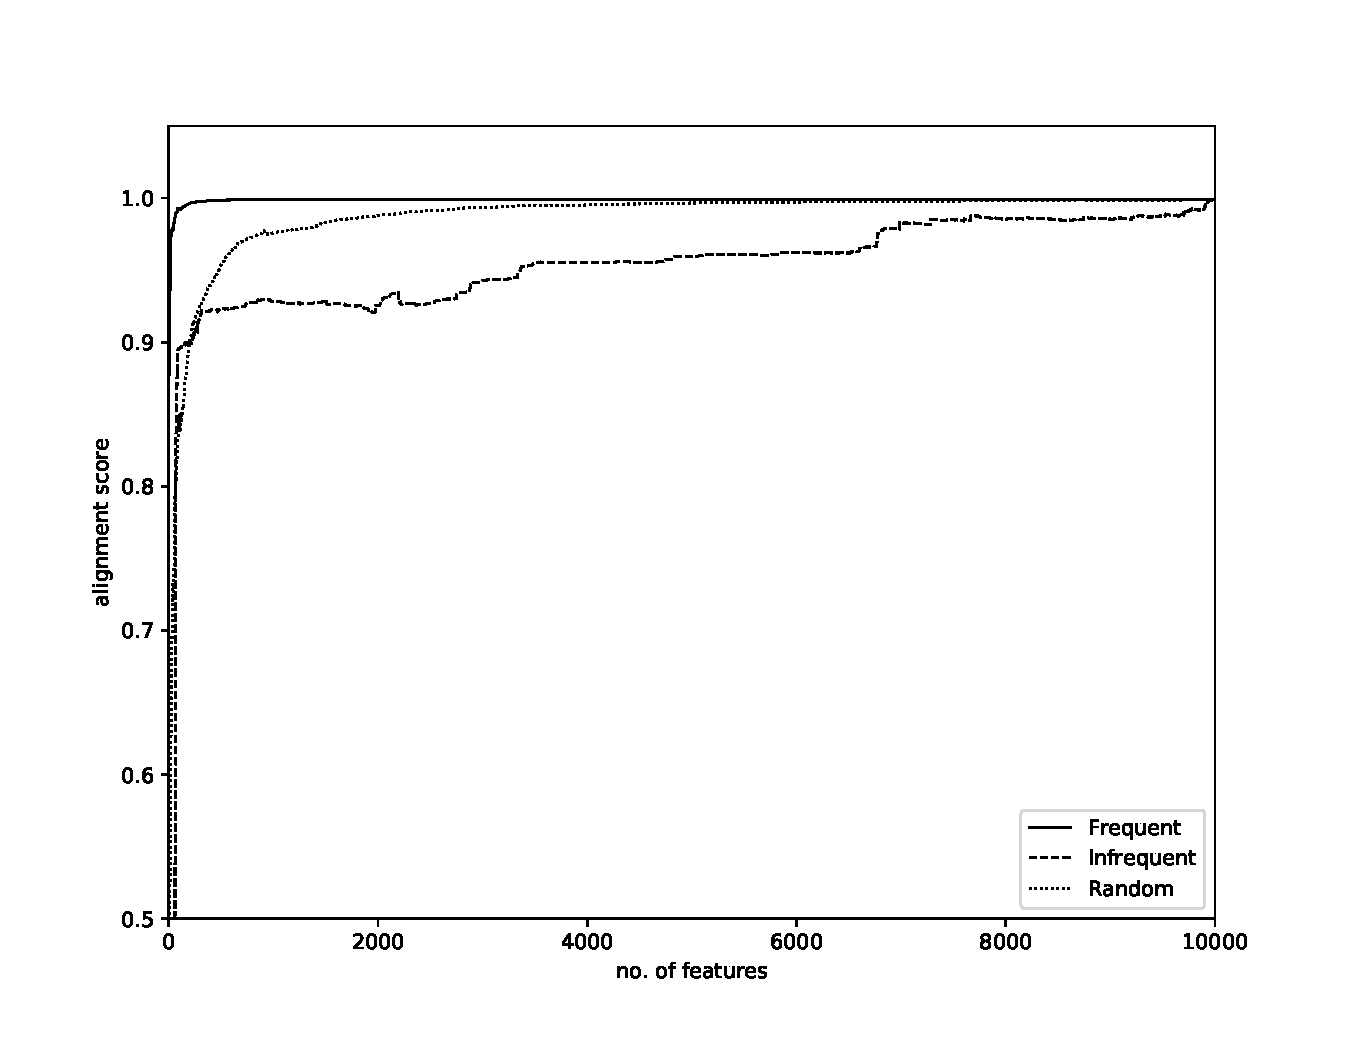
\includegraphics[height = 5.5cm]{../plots/Alignment_scores.pdf}}	
	\subfloat[Lohdi et al.'s]{\raisebox{0.40cm}%
		{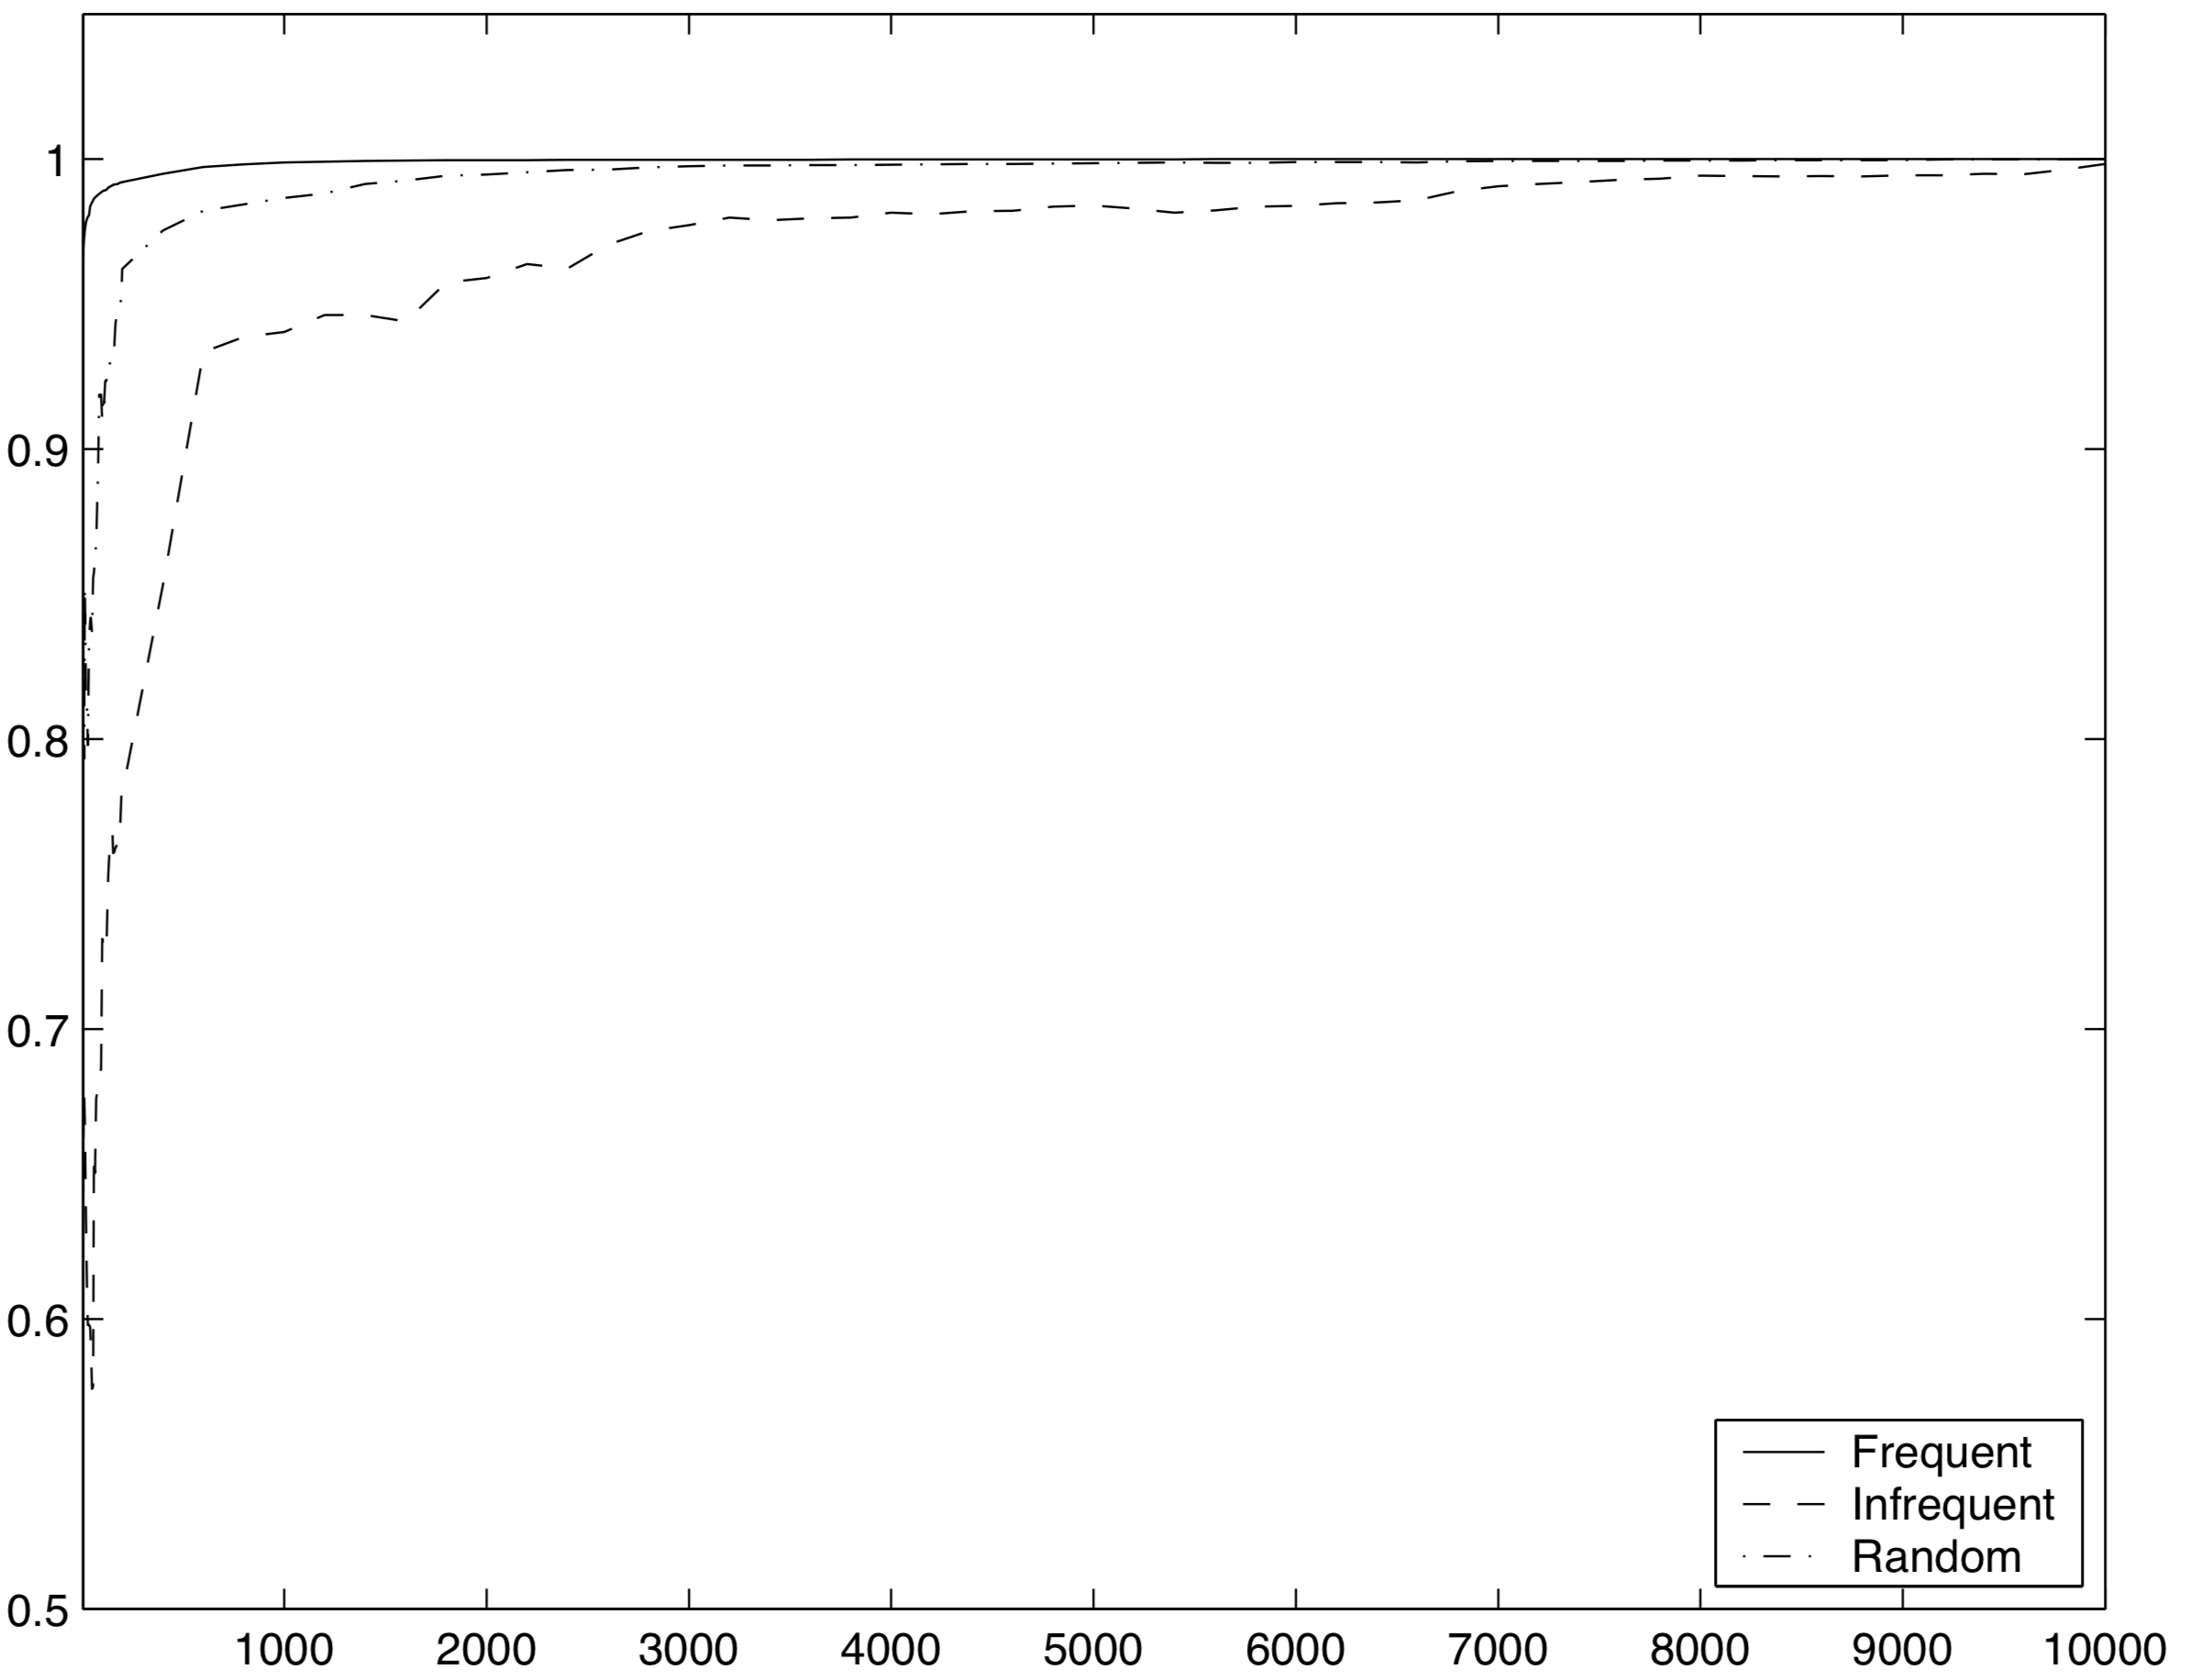
\includegraphics[height = 4.5cm]{../plots/Lodhi_alignment_score.png}}}%
	\caption{Alignment scores for varying the number of vectors $ x $ in the subset $ \tilde{S} $. Lohdi et al.'s figure is shown for comparison.\label{fig:alignment}}
\end{figure}
%table for entire dataset
\begin{table}
	\centering
	\small	
	\begin{tabular}{| c | c | c | c | c | c | c | c |}\hline
		& WK & NGK & NGK  & NGK  & aSSK & aSSK& aSSK \\ 
		&  & $n = 3$& $ n = 4 $ & $ n = 5 $ & $ n = 3 $& $ n = 4 $ & $ n = 5 $ \\ \hline
		earn & 0.98 & 0.98 &  0.98&  0.98 & 0.98 & 0.98 & 0.98 \\ \hline
		acq & 0.97 & 0.95 &  0.95 &  0.96 & 0.95 & 0.95 & 0.95 \\ \hline
		money-fx & 0.79 & 0.77 &  0.79 & 0.77 & 0.77 & 0.8 & 0.78 \\ \hline
		grain & 0.92 & 0.81 &  0.83& 0.82 & 0.84 & 0.86 & 0.8 \\ \hline
		crude & 0.87 & 0.84 &  0.85 & 0.8 & 0.82 & 0.79 & 0.73 \\ \hline
		trade & 0.8 & 0.73 &  0.77 & 0.77 & 0.72 & 0.79 & 0.77 \\ \hline
		interest & 0.8 & 0.72 &  0.73 & 0.75 & 0.79 & 0.8 & 0.77 \\ \hline
		ship & 0.78 & 0.66 &  0.55 & 0.47 & 0.69 & 0.5 & 0.34 \\ \hline
		wheat & 0.79 & 0.86 &  0.84 & 0.8 & 0.8 & 0.8 & 0.76 \\ \hline
		corn & 0.86 & 0.73 &  0.85 & 0.65 & 0.78 & 0.72 & 0.6 \\ \hline	
	\end{tabular}
	\caption{The ten best performing classes from \cite{lodhi} shown with our $ F_1 $ results for WK, NGK and  aSSK using the entire Reuters dataset. For aSSK; $ \lambda = 0.5, x = 3000$\label{tab:full_data} }
\end{table}

%1 big table
\begin{wraptable}[35]{r}{8cm}
	\centering
	\small
	
	\begin{tabular}{| c | c | c | c | c | }
		\hline SSK& $ n $ & Precision & Recall & $ F_1 $   \\ \hline
		
		& 3 & 0.93 & 0.96 & 0.94 (0.785)    \\ 
		& 4 & 0.93 & 0.96 &  0.94  (0.822)  \\
		& 5 & 0.97 & 0.93 & 0.95  (0.867)   \\ 
		& 6 & 0.98 & 0.93 & 0.95 (0.876)    \\
		acq	& 7 & 0.98 & 0.89 & 0.93 (0.864)    \\
		& 8 & 0.99 & 0.80 & 0.93  (0.852)   \\
		& 10 & 0.98 & 0.62 & 0.75  (0.791)   \\
		& 12 & 0.98 & 0.33 & 0.49  (0.791)   \\
		& 14 & 1 & 0.15 & 0.25  (0.774)   \\ \hline
		
		
		
		& 3 & 0.99 & 0.93 & 0.96  (0.925)   \\ 
		& 4 & 0.99 & 0.95 &  0.97  (0.932) \\
		& 5 & 0.99 & 0.96 & 0.97   (0.936)  \\ 
		& 6 & 0.99 & 0.93 & 0.97  (0.936)   \\
		earn& 7 & 0.99 & 0.91 & 0.96 (0.940)    \\
		& 8 & 0.99 & 0.91 & 0.95  (0.934)   \\
		& 10 & 1 & 0.86 & 0.92  (0.927)   \\
		& 12 & 1 & 0.76 & 0.87  (0.931)   \\
		& 14 & 1 & 0.68 & 0.81  (0.936)   \\ \hline
		
		
		& 3 & 0.97 & 0.87 & 0.91  (0.665)   \\ 
		& 4 & 0.98 & 0.64 & 0.88  (0.783)   \\ 
		& 5 & 0.98 & 0.44 &  0.83  (0.779)  \\ 
		& 6 & 0.98 & 0.42 & 0.78   (0.749)  \\ 
		corn& 7 & 0.98 & 0.24 & 0.74  (0.643)  \\ 
		& 8 & 1 & 0.43& 0.59  (0.569)   \\ 
		& 10 & 1 & 0.29& 0.44  (0.582)   \\ 
		& 12 & 0.86 & 0.16& 0.26  (0.618)   \\ 
		& 14 & 0.71 & 0.11& 0.20  (0.702)   \\ 
		\hline
		
		
		& 3 & 0.97 & 0.86 &  0.88  (0.881)  \\ 
		& 4 & 0.98 & 0.80 & 0.91  (0.905)   \\ 
		& 5 & 0.98 & 0.73 &  0.88 (0.936)   \\ 
		& 6 & 0.98 & 0.66 &  0.82  (0.901)  \\
		crude& 7 & 0.98 & 0.60 &  0.73 (0.872)  \\
		& 8 & 1 & 0.43 &  0.67   (0.828) \\ 
		& 10 & 1 & 0.28 &  0.42   (0.764) \\ 
		& 12 & 0.29 & 0.03 &  0.05   (0.709) \\ 
		& 14 & 0.14 & 0.01 &  0.02   (0.761) \\ \hline 
			
	\end{tabular}
\caption{Full range of subsequence lengths used in \cite{lodhi}, who's  $ F_1 $-scores are shown in parentheses.  $  \lambda = 0.5$\label{tab:appendix_ssk_n}}

\end{wraptable}


\begin{figure}
	\centering
	\subfloat[Alignment score between kernels from aSSK and our proposed improvement aSSK ]{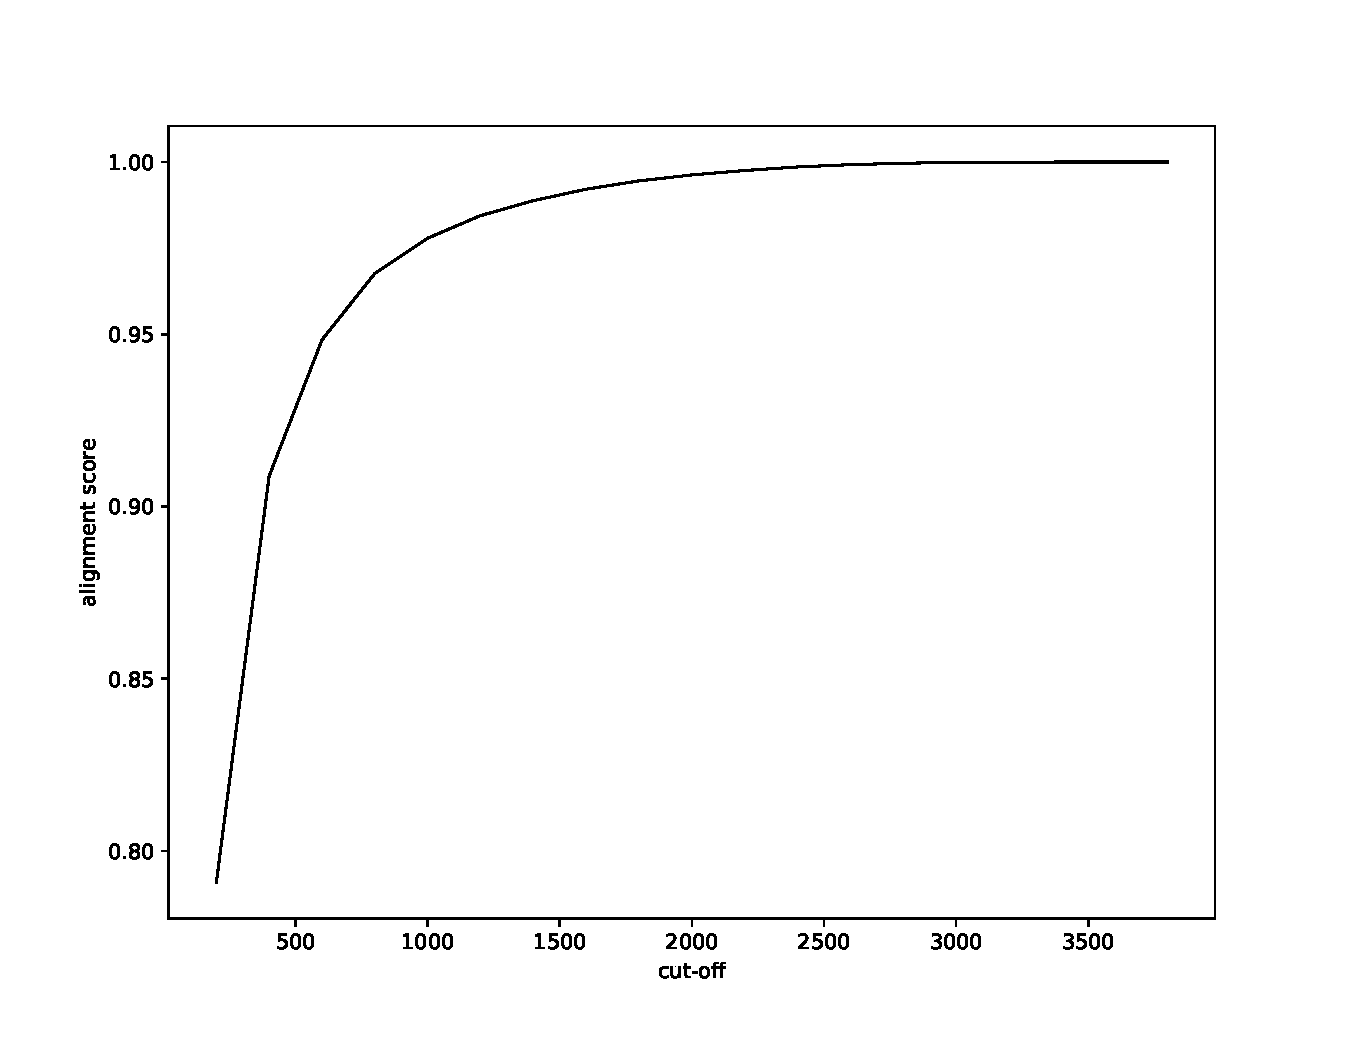
\includegraphics[width=6 cm]{../plots/alignment_score_modification.pdf}}
	\quad\subfloat[Time comparison between computation for our proposed improvment of aSSK and Lodhi et al.'s aSSK.]{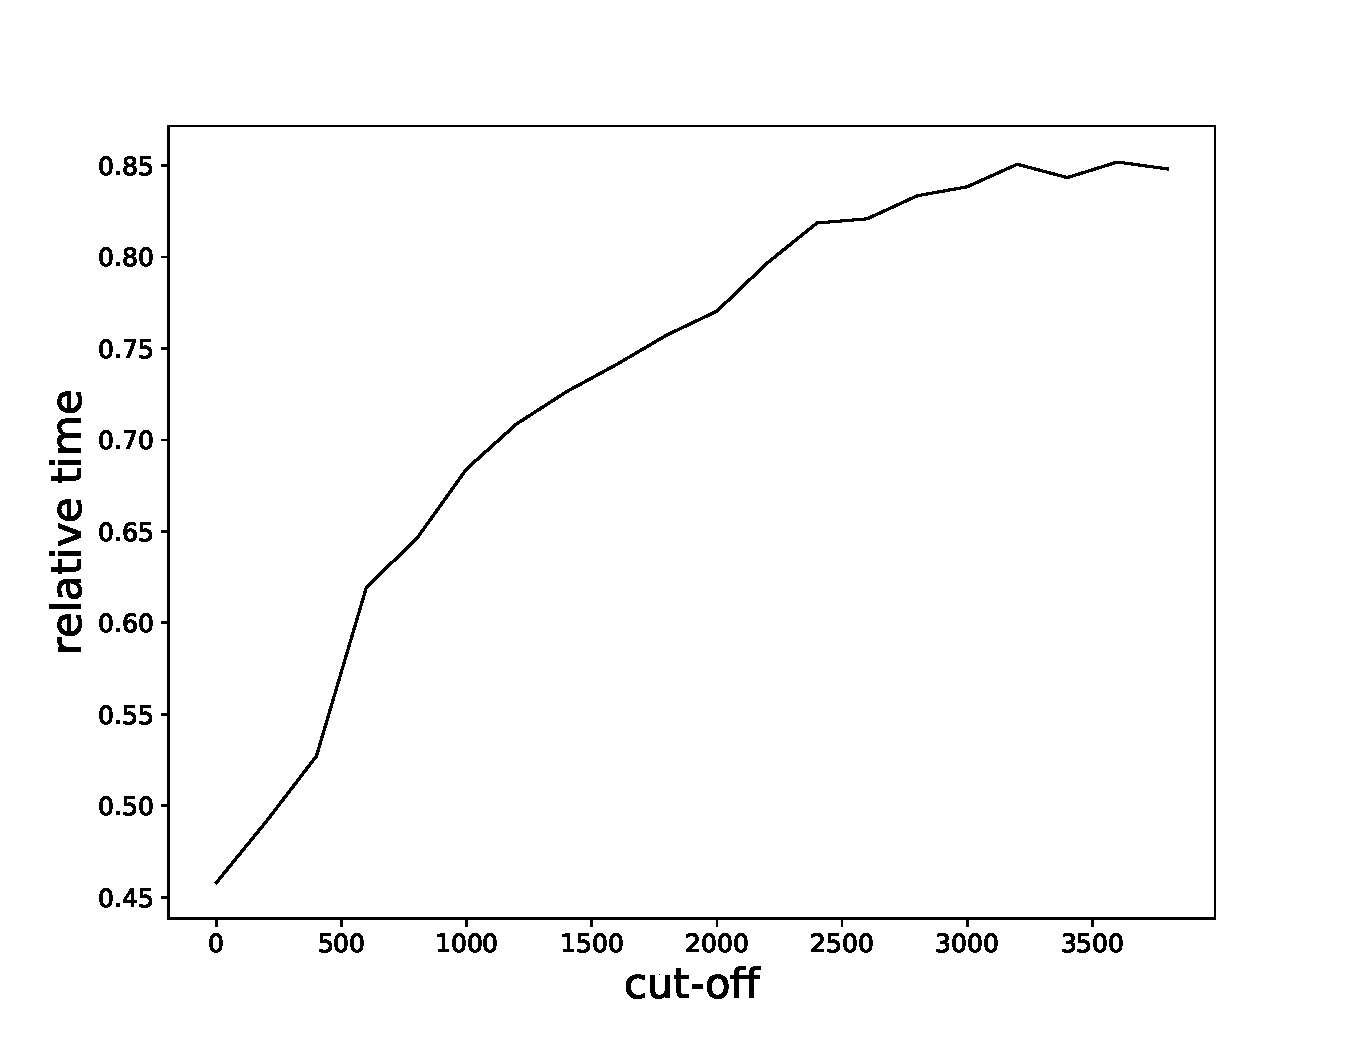
\includegraphics[width=6 cm]{../plots/relative_time.pdf}}
	\caption{Results when comparing our proposed improvement of the aSSK to the aSSK presented in \cite{lodhi}.\label{fig:improved_assk}}
\end{figure}


